% Created 2024-06-06 Thu 16:29
% Intended LaTeX compiler: pdflatex
\documentclass[presentation]{beamer}
\usepackage[utf8]{inputenc}
\usepackage[T1]{fontenc}
\usepackage{graphicx}
\usepackage{longtable}
\usepackage{wrapfig}
\usepackage{rotating}
\usepackage[normalem]{ulem}
\usepackage{amsmath}
\usepackage{amssymb}
\usepackage{capt-of}
\usepackage{hyperref}
\usetheme{Madrid}
\usecolortheme{}
\usefonttheme{}
\useinnertheme{}
\useoutertheme{}
\date{\today}
\title{Отчет об X5 TECH AI HACK}
\usepackage[T1,T2A]{fontenc}

\hypersetup{
 pdfauthor={},
 pdftitle={Отчет об X5 TECH AI HACK},
 pdfkeywords={},
 pdfsubject={},
 pdfcreator={Emacs 29.3 (Org mode 9.6.28)}, 
 pdflang={English}}
\begin{document}

\maketitle


\begin{frame}[label={sec:org0d26e91}]{Чем интересен хакатон X5 TECH AI HACK}
\begin{itemize}
\item Можно видеть, что нейронные сети и языковые модели заменяют собой
классические инструменты программирования, такие как регулярные
выражения, Word2Vec и другие инструменты основанные на императивном
анализе данных.
\item облачные вычисления и сервисы являются 1) ресурсной базой для
вычислений 2) обеспечивают централизованную безопасность
\end{itemize}

Поэтому маскирование приватных данных, поиск именнованных сущностей и
 управление языковыми моделями - это самые частые современные задачи в
 IT.
\end{frame}
\begin{frame}[label={sec:orge8222f8}]{Маскирование: постановка}
Вход: текст

Выход: этот текст с заменененными сущностями (телефоны, фамилии,
 адреса \ldots{})  на похожие.

Дополнително: иметь возможность обратной замены, устойчивой к взлому.
\end{frame}
\begin{frame}[label={sec:orgef3c8b8}]{Проблемы}
\begin{itemize}
\item Маленький датасет с ошибками
\item нет доступа к Интернету
\item 8GB RAM, только CPU
\end{itemize}
\end{frame}
\begin{frame}[label={sec:org67b5f77}]{Маскирование: Baseline}
BERT English 110M параметров - чествительная к регистру
\begin{enumerate}
\item без токенайзера
\item Обучение NER - 400 epochs с 2e-5 lerning rate
\item неразмеченный текст подается модели посимвольно
\end{enumerate}

текст разбивается на токены в 1 символ и помечается в BIO
\end{frame}
\begin{frame}[label={sec:orgb7a192c}]{BERT - что это?}
BERT - языковая модель на основе Transformer на одном кодировщикe.
\begin{itemize}
\item Вход - фиксированная строка, выход - фиксированная строка.
\item Tokenizer c WordPiece - обученный отдельно.
\item предобучен на Masked LM и Next Sentence Prediction (NSP)
\end{itemize}
\begin{center}
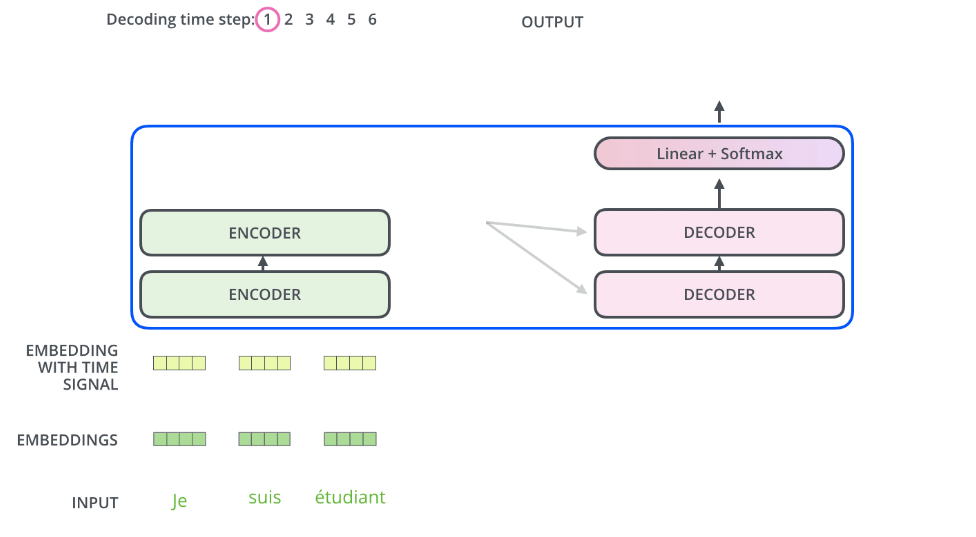
\includegraphics[width=.9\linewidth]{./imgs/image-2.png}
\end{center}











\url{./imgs/image-2.gif}


This technique allows certain out-of-vocabulary words to be
 represented as multiple in-vocabulary “sub-words”, rather than as the
 [UNK] token.  "clockwork", - clock + work
\end{frame}

\begin{frame}[label={sec:org3799d0e}]{Маскирование: простые решения}
\begin{enumerate}
\item Использование слов, а не символов -  предобученного токенизатора
\item Обучение Tokenizer на словах
\item Использование предобученной модели и токенайзера на русском корпусе
\item DataCollatorForTokenClassification вместо самописного
\item при обучени устранение дисбаланса классов
\end{enumerate}
\end{frame}

\begin{frame}[label={sec:orgebcb938}]{Маскирование: победившие решения}
\begin{itemize}
\item использование bert-base-multilingual-cased
\item регулярные выражения + LLM NER + поиск по словарю
\begin{itemize}
\item найденные позиции помечаются
\end{itemize}
\item xml-roberta-large-ner-russian
\item удаление лишних пробелов знако пунктуцаии улучшает NER.
\end{itemize}
\end{frame}
\begin{frame}[label={sec:orgb56a671},fragile]{Маскирование: наше решение}
 \begin{itemize}
\item без дообучения DeepPavlov/ner\_rus\_bert + regex выражения
\end{itemize}

Результатирующая точность: 0.41 - низкий. Времени не хватило на
 выяснение причин.
\begin{verbatim}
link_pattern = r'https?://\w*\.\w*/'
phone_pattern = r"((8|\+7)[\- ]?)?(\(?\d{3}\)?[\- ]?)?[\d\- ]{7,10}" # r"^((8|\+7)[\- ]?)?(\(?\d{3}\)?[\- ]?)?[\d\- ]{7,10}$"
email_pattern = r'\b[A-Za-z0-9._%+-]+@[A-Za-z0-9.-]+\.[A-Z|a-z]{2,}\b' # "[^@]+@[^@]+\.[^@]+"
date_pattern = r'\b\d{2}\.\d{2}\.\d{4}\b'
num_pattern = r'\b\w*[0-9]+\w*\b'
acr_pattern = r'\b[A-Z]{3}\b'
\end{verbatim}
\end{frame}

\begin{frame}[label={sec:orgec393f8}]{Галлюцинации: постановка}
Вход: контектс, вопрос, ответ.

Выход: метка 0/1 ответ правильный или нет.

Дополнительно: сделать из решения качественный программный продукт.
\end{frame}
\begin{frame}[label={sec:orgbc883a3}]{Галлюцинации: Baseline}
BERT English 110M параметров - нечувствительная к регистру
\begin{enumerate}
\item токенайзер - huggingface.TFBertTokenizer
\item дополнительный слой с выходом на 2 нейрона
\item loss = nn.CrossEntropyLoss() - бинарная классификация
\begin{itemize}
\item Вход: "summary: '' | question: '' | answer: ''
\item Выход: следующее слово - метка
\end{itemize}
\end{enumerate}
\end{frame}
\begin{frame}[label={sec:org4927162}]{Галлюцинации: победившие решения}
\begin{itemize}
\item\relax [CLS] + summary + [SEP] + question + [SEP] + answer + [SEP].
\item token\_type\_ids mask = 1 для ответа
\item Стеккинг нескольких LLM и простой классификатор для объединения
\item Генерация датасета на базе RussianNLP/wikiomnia
\item Выделение признаков - сомнительно
\item Применение Saiga\_8b\_q4 и DeepPavlov/rubert-base-cased
\item Проверка выхода Baseline решения и добавление второй LLM
\end{itemize}









\url{https://huggingface.co/docs/transformers/glossary\#token-type-ids}
\end{frame}
\begin{frame}[label={sec:org3d1eebd}]{Галлюцинации: наши решения}
\begin{enumerate}
\item Saiga Llama3 8B + IPEX квантование - простой prompt engineering
\item Knewledge Distilation 0.902 - Малая модель учится повторять большую
\begin{itemize}
\item cross-entropy loss function между парамтртризорованным ответом учителя и студента
\item студент: cointegrated/rubert-tiny2
\item учитель: DeepPavlov/rubert-base-cased
\end{itemize}
\end{enumerate}











a small model is trained to mimic a pre-trained, larger model (or ensemble of models)
\end{frame}

\begin{frame}[label={sec:org836a163}]{Недостатки хакатонов}
\begin{itemize}
\item Датасеты с ошибками, нужно повторить ошибки чтобы победить
\item Организаторы дают свой подход и если не следовать ему это почти 100\% самоубийство, так как временя ограничено
\item Заходить на хакатон нужно только с полной коммандой и в первые дни после объявления
\item Важна только скорость любой ценой, чем не контер страйк?
\item В угоду скорости приходится жертвовать безопасностью, а это имеет долгосрочный характер.
\item Главная сложность это понять что вообще организаторы ожидают, что должно быть сделано.
\item Напряжения сил требуется для победы больше, что приз.
\item Залог победы - хорошая большая команда
\end{itemize}
\end{frame}

\begin{frame}[label={sec:org6b4d63e}]{Достоинства и возможности хакатонов}
\begin{itemize}
\item Найти команду и партнеров
\item Отбросить медленные неэффективные подходы
\item Попробовать командную работы
\item Узнать новое и современное
\item Узнать эффективные подходы от других команд
\end{itemize}
\end{frame}

\begin{frame}[label={sec:orgc4e07d4}]{Командная работа}
\begin{itemize}
\item Общий чат без созвонов - один из лучших форматов.
\item Любые напоминания о необходимости работать убивают желание работать.
\item Письменный отчет каждый день о проделанной работе как средство проверки на бездельника. Но дополнительная нагрузка.
\item Бездельникам нужно раздавать четкие задачи раньше
\item Нет отчета - либо бездельник, либо загнал себя и не успевает.
\item Правила которые ты ждешь от других лучше доносить персонально с подтверждением и всеми возможными вариантами событий.
\item Со временем люди работают меньше, а не больше. Поэтому нужно оценивать по первичной работоспособности.
\item Человек с пустым гитхаб аккаунтом не программист, а аналитик или ученый.
\end{itemize}
\end{frame}

\begin{frame}[label={sec:org9e03a10}]{Допущенные ошибки}
\begin{itemize}
\item Маленькая команда из недосаточно свободных людей
\item Использование масштабных подходов с полой заменой Baseline
\item Отсутствие подготовленного GPU у каждого в команде
\item Дообучение и finetuning и ансамблирование, это главные навыки всех хакатонов, кооторыми нужно владеть в совершенстве
\end{itemize}
\end{frame}


\begin{frame}[label={sec:org08dab5c}]{Интересные факты}
\begin{itemize}
\item Предобработка текста для LLM улучшает качество
\item Можно использовать ансамбли из малых языковых моделей
\item Knewledge distillation как эффективный метод дообучения малых языковых моделей
\item Галлюцинации это не факт чекинг.
\item Языковые модели эффективнее регулярных выражений, потому что на практике риск ошибки и взлома не критичен.
\end{itemize}
\end{frame}
\end{document}
